\section{Opdrachtbeschrijving}
In het kader van ons bachelorproject ontwikkelden we een wagentje dat autonoom zo snel mogelijk een raceparcours kan afleggen. Dit parcours bestaat uit een zwarte ondergrond afgebakend door volle witte lijnen en een witte stippellijn in het midden, een voorbeeld hiervan ziet u in figuur~\vref{fig:parcoursvoorbeeld}. Ons wagentje mag niet buiten de volle witte lijnen van het parcours treden. Op het traject bevinden zich verschillende RFID-tags die door het voertuig ingelezen moeten worden. Eveneens moest er een manier voorzien worden om de snelheid van het voertuig te meten. De ingelezen tags en opgemeten snelheid moesten ten slotte nog verzonden worden naar een Raspberry Pi.\\
\begin{figure}[H]
	\centering
	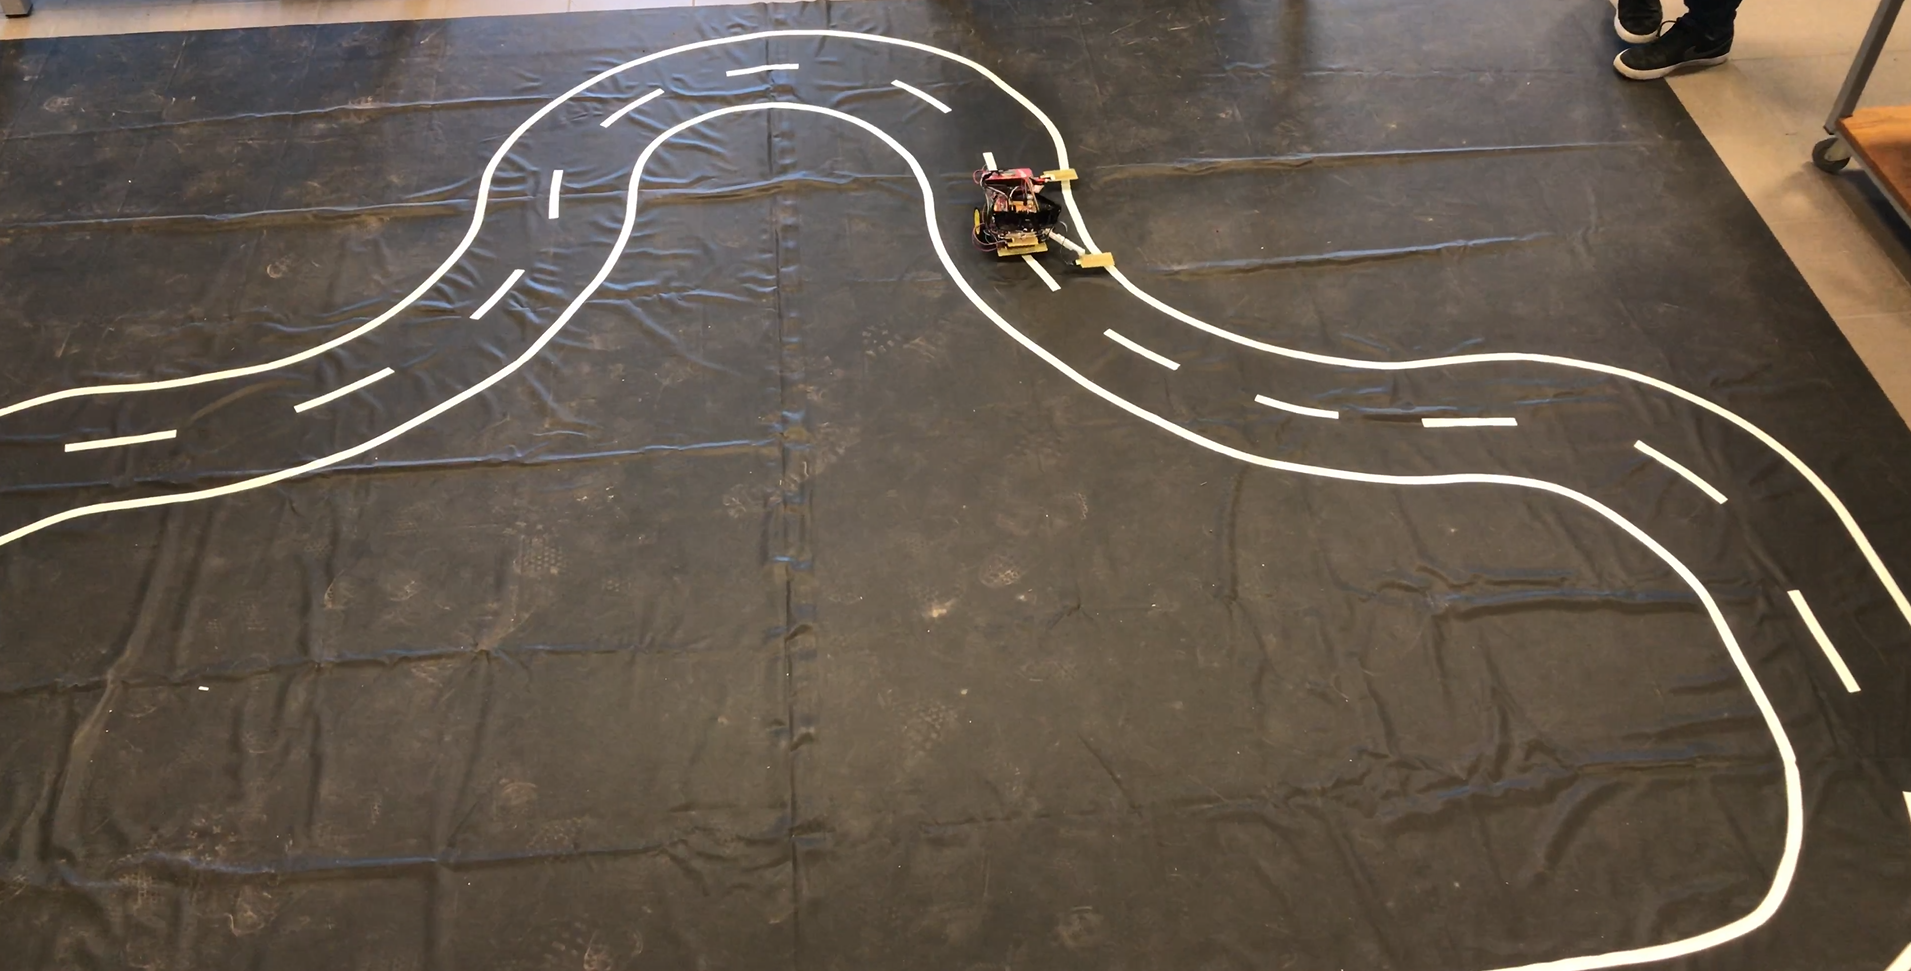
\includegraphics[width=\textwidth]{parcoursvoorbeeld.png}
	\caption{Voorbeeld van een parcours}
	\label{fig:parcoursvoorbeeld}
\end{figure}
\subsection{Hardware}
We kregen reeds een wagentje met twee motoren en een batterij om het project mee aan te vangen.
Voor het prototypen en testen mochten we gebruik maken van een voorziene Arduino Uno met motor shield op dit wagentje. Een belangrijk deel van de opdracht bestond er uit deze Arduino \'en motor shield te vervangen door \'e\'en custom board.
Qua hardware moesten we dus nog de custom board ontwikkelen, sensoren voorzien en uiteraard ook modules aanschaffen voor (Bluetooth) communicatie met de RPi en het inlezen van RFID-tags.\\
\subsection{Software}
De besproken hardware moest natuurlijk ook correct aangestuurd worden door software. Dit gebeurt aan de hand van Arduino-code ondersteund door vrij verkrijgbare, of zelfgeschreven C/C++ libraries. We schreven dus zelf code voor het aansturen van de motoren, het inlezen van sensoren, communicatie met Raspberry Pi,...
Aan de kant van de Raspberry Pi moesten we verbinding maken met ons wagentje en de data die doorgestuurd werd af printen op het scherm.


\section{Doelstellingen}
De belangrijkste doelstellingen van ons project zijn dus als volgt samen te vatten:
\begin{itemize}
	\item Voertuig autonoom en zo snel mogelijk een parcours laten afleggen
	\item Custom board ontwerpen om Arduino en motorshield te vervangen
	\item Snelheid van het wagentje meten
	\item RFID-lezer voorzien voor het uitlezen van tags op het parcours
	\item Communicatie (Bluetooth) tussen Arduino en Raspberry Pi 3 realiseren
\end{itemize}
\section{Structuur}
We beginnen dit verslag met een bespreking van onze planning, taakverdeling en gemaakte onkosten. Daarna behandelen we de gebruikte hardware en software om deze aan te sturen in meer detail. Vervolgens overleggen we de problemen en moeilijkheden die we doorheen het project ondervonden. Hierna volgt nog een evaluatie van onze coach, Bert Cox. Ten slotte eindigen we met een besluit omtrent het project waarin we samenvatten wat we realiseerden, wat we hebben bijgeleerd, wat er beter kan/kon,...